\documentclass[a4paper]{article}

\usepackage[english]{babel}
\usepackage[utf8]{inputenc}
\usepackage{amsmath}
\usepackage{graphicx}
\usepackage{float}
\usepackage[colorinlistoftodos]{todonotes}
\newtheorem{theorem}{Theorem}[section]
\newtheorem{lemma}[theorem]{Lemma}


\title{Equitable Stable Marriage - Term Project\\Social Computing - Fall 2018}

\author{Swapna Mukrappilly\\Jason Trout\\Zach Southwell\\Joshua Musick}

\date{\today}

\begin{document}
\maketitle

\begin{abstract}
Short summary about how we approached solving an NP-Hard Problem...
\end{abstract}

\section{Introduction}
\label{sec:introduction}

Explain the context of the experiment here. Why is condensed matter physics interesting or important?
Optional things you could talk about (but don't have to -- this is up to you): transistors, computers, Quantum computers, fundamental knowledge (e.g. the resistance quantum).

Briefly explain what methods you will use in the experiment, and what values you will extract from the data.

For this section and all following sections: If you refer to an equation, previous result or theory that is not regarded as common knowledge, then cite the source (article or book) where you found this. For example, you can cite the Nano 3 Lecture notes \cite{nano3}.

%%%%%%%%%%%%%%%%%%%%%%%%%%%%%%%%%%%%%%%%%%%%%%%%%%%%%%%%%%%%%%%%%%%%%%%%%%%%%%%%%%%%%%%%%%%%

\section{Background}
\label{sec:background}

\subsection{Stable Marriage Problem}
The Stable Marriage Problem can be described as follows: We are given a set of unmarried men and women. The cardinality of each gender in this set is equal. Each person in this set provides an ordered preference list which contains all members of the opposite gender. We want to produce a matching such that:
\begin{itemize}
    \item Each member of the set is matched with a member of the opposite gender.
    \item There are no blocking pairs. That is to say, there are no two pairs such that the man in one pair and the woman in another pair both prefer each other to their current partners.
\end{itemize}
There is always at least one stable matching. (TODO: provide brief proof here?)

The Gale-Shapely algorithm is effective in finding a stable matching given any valid problem set. An interesting property of this algorithm is that it is strongly biased in favor of one of the genders. For the optimal group, each and every member of that group is guaranteed to be matched with the best possible partner for any stable matching. Alternately, each member of the non-optimal group is guaranteed to be matched with the worst possible partner for any stable matching.

\subsection{Equitable Matching}
The systematic bias that the Gale-Shapely algorithm applies toward the optimal group is not an equitable solution. How can we find a more equitable solution?

First, it's important to define what property we are looking for in this solution. Let the function $score(p, m)$ be defined as the position of a person $p$'s assigned match $m$ in their preference list. So for example, if a man $M_1$ has the preference list [$W_3$, $W_1$, $W_4$, $W_2$], and ($M_1$, $W_3$) are matched in some matching, then score($M_1$, $W_3$) is $0$. Clearly, a lower individual score is better.

One approach to finding a more equitable matching might be to find a stable matching where the sum of the scores for all men is closest to the sum of all scores for women. One might argue that this would be the most equitable arrangement because we would be minimizing the advantage of one gender over another in our matching.

A shortfall of this method however, is that such a stable marriage could actually lead to both genders having a less favorable overall matching. As an example, suppose some man-optimal matching produced a cumulative score of 25 for the men and 30 for the women. Now let's suppose that we were able to find a stable marriage such that each gender had equivalent cumulative scores of 35. By the criteria we've described above, this is a more equitable arrangement, but it turns out that each group is less happy with thier partner than with the man-optimal matching.

\textcolor{red}{IS THIS TRUE? The man optimal would be the woman-pessimal, and therefore, all women could only improve their matching, and therefore their cumulative score can only improve.}

\textcolor{blue}{Ah, you're right... I think it's still a valid point but my example is wrong... How about this: Suppose some man-optimal matching produces a cumulative score of 20 for the men and 30 for the women. Suppose the woman-optimal matching for the same set produces the opposite: a cumulative score of 20 for the women, but 30 for the men. Now suppose that we find the the most balanced matching produces cumulative scores of 28, 28. But what if there were a matching that produced cumulative scores of 23, 27, wouldn't that be better, even if it's less balanced? }

Instead, our criteria for finding the `equitable' matching is a matching that minimizes the total cumulative score for all participants of the matching. This optimal matching may turn out to be more favorable to one gender, but it cannot be less favorable than one of the man/woman optimal matchings. (This is trivially true because the least favorable matching for any group/individual is one of the man/woman optimal matchings)

Unfortunately we found out that this is an NP hard problem to solve. (TODO: add some explanation about why the problem is intractable)

The optimal solution requires one to traverse all possible stable matchings. For each stable matching, we have to calculate the cumulative score and record the best value.

\section{Experiment}
\subsection{Equitable Metrics}
Describe what an equitable matching is, and how we are quantifying it in our program.

\subsection{Brute Force Solution}
We initially developed a brute-force algorithm to compute all stable matchings in a problem set. Here's what that algorithm looked like initially:
\begin{enumerate}
    \item Use the Gale-Shapely algorithm to calculate the man-optimal stable matching
    
    \item Use the Gale-Shapely algorithm to calculate the woman-optimal stable matching
    
    \item For each person, build a reduced preference list. This list starts from the preference list, but values which occur prior to the optimal match, or after the pessimal match are removed. For example, the following problem set has these preference lists:


\begin{table}[H]
\centering
\caption{}
\begin{tabular}{lllll}
$M_1$: & $W_1$ & $W_4$ & $W_2$ & $W_3$ \\
$M_2$: & $W_3$ & $W_2$ & $W_4$ & $W_1$ \\
$M_3$: & $W_2$ & $W_1$ & $W_3$ & $W_4$ \\
$M_4$: & $W_1$ & $W_4$ & $W_3$ & $W_2$ \\
\\
$W_1$: & $M_2$ & $M_3$ & $M_1$ & $M_4$ \\
$W_2$: & $M_3$ & $M_1$ & $M_4$ & $M_2$ \\
$W_3$: & $M_4$ & $M_2$ & $M_3$ & $M_1$ \\
$W_4$: & $M_1$ & $M_4$ & $M_2$ & $M_3$ \\
\end{tabular}
\end{table}

And produces these `reduced preference lists':
\begin{table}[H]
\centering
\caption{}
\begin{tabular}{lllll}
$M_1$: & $W_1$ & $W_4$ & &       \\
$M_2$: & $W_3$ & $W_2$ & $W_4$ & $W_1$ \\
$M_3$: & $W_2$ & & &          \\
$M_4$: & $W_4$ & $W_3$ & &       \\
                        \\
$W_1$: & $M_2$ & $M_3$ & $M_1$ &    \\
$W_2$: & $M_3$ & & &          \\
$W_3$: & $M_4$ & $M_2$ & &       \\
$W_4$: & $M_1$ & $M_4$ & &       \\
\end{tabular}
\end{table}

    \item Permute over all possible arrangements of the reduced preference lists. This is the `brute-force' part. For each permutation:
    \begin{enumerate}
        \item Calculate whether the matching is stable. Many of the matchings calculated in this manner are NOT stable.
        \item For unstable matches, skip to the next permutation.
        \item For stable matches, calculate the cumulative score of the match (using the full preference list) and record the lowest value.
    \end{enumerate}

\end{enumerate}

With this method, problem sets quickly became intractable as the number of pairs approached a 20-30, although this varies based on how much the preference lists can be pruned. It's not unreasonable for randomized test cases of this size to only produce one or two possible matchings, in which case the problem set might complete very quickly, while another problem set of the same size might never complete. (TODO: maybe show some data on run-times with different data sets of the same size?)

\subsection{Heuristics}
\subsubsection{Feasible Matches - Upper and Lower Bounds}
Describe how we used the man-optimal and woman-optimal solutions to prune our "feasible match" list by applying the man-optimal solution as the upper bound for men, and the woman-optimal solution as the lower bound for men, and vice versa...

\subsubsection{Complimentary Feasible Matches}
We were able to improve on this algorithm slightly by removing more items from preference lists. For instance, if $M_2$ does not appear in $W_2$'s reduced preference list, then the matching ($M_2$, $W_2$) is not possible and so $W_2$ should not appear in $M_2$'s reduced preference list. This strategy helped to remove many matchings that were invalid when the reduced preference list had many items between the optimal and pessimal results. (TODO: do we want to collect some data on how much better we did with these improvements?)

Using this strategy, we can further refine our `reduced preference list' to the following:
\begin{table}[H]
\centering
\caption{}
\begin{tabular}{lllll}
$M_1$: & $W_1$ & $W_4$ & &       \\
$M_2$: & $W_3$ & $W_1$ \\
$M_3$: & $W_2$ & & &          \\
$M_4$: & $W_4$ & $W_3$ & &       \\
                        \\
$W_1$: & $M_2$ & $M_1$ &    \\
$W_2$: & $M_3$ & & &          \\
$W_3$: & $M_4$ & $M_2$ & &       \\
$W_4$: & $M_1$ & $M_4$ & &       \\
\end{tabular}
\end{table}

\subsubsection{Unique Matching}
Describe how we also applied a pruning heuristic based on whether we had a unique matching between a specific man and woman, meaning that was their ONLY feasible match.  In this case, that man would be removed from all other women's feasible lists, and the woman would be removed from all other men's feasible lists.

\subsection{Rotations}
Can we do any better? After implementing the brute-force approach above, we tried again using a strategy of match rotations detailed by Gusfield/Irving \cite{gusfield} to efficiently traverse the set of all stable matchings.

To explain this approach, let's define some functions which can be applied to any existing stable marriage:
\begin{itemize}
    \item Define $currentMatch(p)$ to be the current match for person $p$
    \item Define $nextMatch(p)$ as follows: the first person in the preference list for person $p$, who prefers $p$ over their current partner. Necessarily, $nextMatch(p)$ must follow $currentMatch(p)$ in $p$'s preference list, otherwise the matching would not be stable. Of course, it is also possible that $nextMatch(p)$ does not exist. This is the case for any person matched with their pessimal match. As an example, looking at the problem set shown in table 3, we can use the reduced preference list to identify $nextMatch(p)$.  For the man-optimal matching, $currentMatch(M_2) = W_3$, and $nextMatch(M_2) = W_1$.
    \item Define $consolationMatch(p)$ as the $currentMatch(nextMatch(p))$. In other words, the current match of $nextMatch(p)$. For our example shown in table 3, suppose we are taking the man-optimal match where $currentMatch(M_1) = W_1$, then $consolationMatch(M_1) = M_4$.
    \item Define a rotation in a matching as any ordered subset of matched pairs in a matching such that: for each matched pair $i$: ($0 \leq i \leq r)$, $consolationMatch(M_i) = consolationMatch (M_{i+1})$ where $r$ is the cardinality of the subset of matched pairs and $i+1$ is taken modulo $r$. Using the example from table 3: the set of men has the following rotation: ($M_1, M_4, M_2$): \\
    $consolationMatch(M_1) = M_4$ \\
    $consolationMatch(M_4) = M_2$ \\
    $consolationMatch(M_2) = M_1$
    \item Let $M$ be a stable matching and $p$ be some rotation exposed in $M$. Then define $M / p$ as the matching that results from re-assigning all men in the rotation to $nextMatch(M_i)$

\end{itemize}

\begin{lemma}
If $M$ is a stable matching and $p$ is a rotation in $M$, then $M / p$ is a stable matching.
\end{lemma}
Proof: Suppose $(m, w)$ is a blocking pair in $M / p$. All women in $M / p$ either have the same partner in $M$ or a new partner that they prefer more, so if $w$ prefers $m$ in $M / p$, then $w$ prefers $m$ in M. So $m$ must be in the rotation $p$ otherwise $(m, w)$ would be a blocking pair in $M$. So $m$ prefers $w$ less than his matching in $M$, but more than his matching in $M / p$, but this violates the definition of the $nextMatch(m)$ function used to define a rotation.

\subsubsection{The Set of All Stable Matchings as a Distributive Lattice}

A stable matching can be expressed as a vector of $score(M_i, currentMatch(M_i))$
The set of stable matchings expressed in this way forms a distributive lattice. Consider the following problem set:

\begin{table}[H]
\caption{}
\begin{tabular}{llllll}
$M_1$: & $W_1$ & $W_3$ & $W_2$ & $W_4$ & $W_5$ \\
$M_2$: & $W_5$ & $W_1$ & $W_3$ & $W_2$ & $W_4$ \\
$M_3$: & $W_2$ & $W_3$ & $W_5$ & $W_4$ & $W_1$ \\
$M_4$: & $W_3$ & $W_1$ & $W_5$ & $W_4$ & $W_2$ \\
$M_5$: & $W_4$ & $W_5$ & $W_2$ & $W_3$ & $W_1$ \\
\\
$W_1$: & $M_3$ & $M_2$ & $M_4$ & $M_5$ & $M_1$ \\
$W_2$: & $M_2$ & $M_5$ & $M_4$ & $M_1$ & $M_3$ \\
$W_3$: & $M_5$ & $M_3$ & $M_1$ & $M_4$ & $M_2$ \\
$W_4$: & $M_4$ & $M_1$ & $M_3$ & $M_5$ & $M_2$ \\
$W_5$: & $M_4$ & $M_2$ & $M_3$ & $M_5$ & $M_1$ \\
\end{tabular}
\centering
\end{table}

In this scenario, the man-optimal matching can be expressed as: $[0,0,0,0,0]$. In other words, the man-optimal matching in this case has all men assigned to the first woman on his preference list. If we use the rotation algorithm described above, we can traverse the entire lattice of stable matchings from the man-optimal to the woman optimal. In this case, there are 8 possible stable matchings, shown in the Hasse diagram below:

\begin{figure}[h]
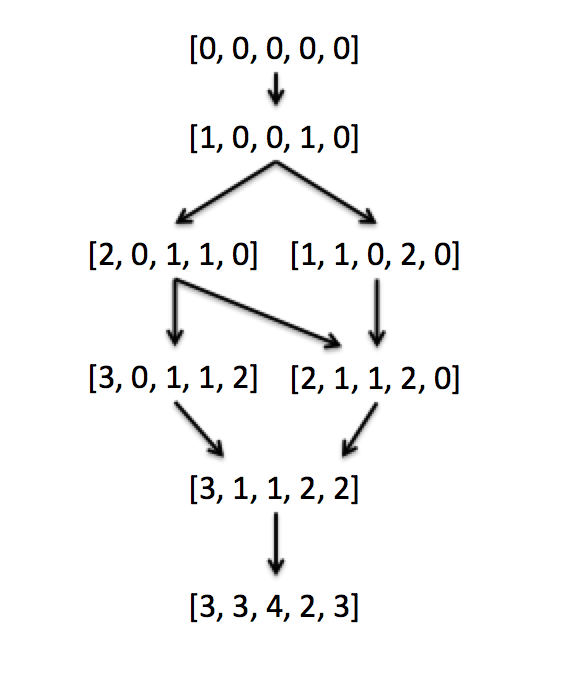
\includegraphics[scale=0.6]{stable_matching_poset.png}
\centering
\end{figure}

\subsubsection{Rotation algorithm}
The algorithm using rotations to traverse through the lattice of all stable matchings:

\begin{enumerate}
    \item Use the Gale-Shapely algorithm to calculate the man-optimal stable matching
    
    \item Use the Gale-Shapely algorithm to calculate the woman-optimal stable matching
    
    \item Use the man-optimal and woman-optimal matchings to identify pairings that are not feasible:
    \begin{enumerate}
        \item For a man $M$, any woman $W$ that occurs in $M$'s preference list prior to $M$'s optimal match or after $M$'s pessimal match is not feasible.
        \item Likewise, for a woman $W$, any man $M$ that occurs in $W$'s preference list prior to $W$'s optimal match or after $W$'s pessimal match is not feasible.
    \end{enumerate}

    \item For each person, build a reduced preference list by taking the full preference list, then for each non-feasible pairing($M_i$, $W_j$), remove $M_i$ from the reduced preference list of $W_j$ and remove $W_j$ from the reduced preference list of $M_i$

    \item Calculate the cumulative $score$ for all people in the man-optimal matching.

    \item Starting with the man-optimal matching, execute the following:

    \item Identify any rotations in the given set. For each rotation found:
    \begin{enumerate}
        \item Take the matching produced by applying the rotation.
        \item If the rotation has been visited already, return.
        \item Calculate the cumulative $score$ for all people in the matching. If the score is the lowest found so far, record the score.
        \item Repeat step 7 with the rotated matching.
    \end{enumerate}
\end{enumerate}

This algorithm was able to calculate optimal matching much more efficiently and handled larger data sets. Still, traversing all possible matchings becomes more and more computationally expensive as the number of pairs grows to more than a thousand. I was able to find the optimal match 1000 pairs in about 4 minutes, while 2000 pairs took around 15 minutes. (TODO: Maybe we can do some benchmarking here to be more specific?) (Also, one interesting thing I found is that as the number of pairs goes up, the cumulative score of the optimal match becomes much better than the cumulative score of either the man-optimal or woman-optimal matches. It may be interesting to see how the average equity score / average man/woman optimal score as a function of the number of pairs)

(Another interesting idea, although I don't know if we have any space to discuss, is that you could just traverse down one chain of the lattice and maybe find a reasonably good option without necessarily having to traverse every matching in the lattice)


%%%%%%%%%%%%%%%%%%%%%%%%%%%%%%%%%%%%%%%%%%%%%%%%%%%%%%%%%%%%%%%%%%%%%%%%%%%%%%%%%%%%%%%%%%%%%

\section{Results}
Show our results, meaning some sample equality metrics for a man-optimal vs woman-optimal and our matching...

\begin{description}
\item[Word] Definition
\item[Concept] Explanation
\item[Idea] Text
\end{description}

We hope you find write\LaTeX\ useful, and please let us know if you have any feedback using the help menu above.

\begin{thebibliography}{9}
\bibitem{gusfield}
  Dan Gusfield and Robert W. Irving,
  \emph{The Stable Marriage Problem: Structure and Algorithms 1989}.

\end{thebibliography}
\end{document}
� 2018 GitHub, Inc.
Terms
Privacy
Security
Status
Help
Contact GitHub
Pricing
API
Training
Blog
About

